%  LaTeX support: latex@mdpi.com
%  In case you need support, please attach all files that are necessary for compiling as well as the log file, and specify the details of your LaTeX setup (which operating system and LaTeX version / tools you are using).

% You need to save the "mdpi.cls" and "mdpi.bst" files into the same folder as this template file.

%=================================================================
\documentclass[journal,article,submit,moreauthors,pdftex,10pt,a4paper]{mdpi} 

%--------------------
% Class Options:
%--------------------
% journal
%----------
% Choose between the following MDPI journals:
% actuators, admsci, aerospace, agriculture, agronomy, algorithms, animals, antibiotics, antibodies, antioxidants, applsci, arts, atmosphere, atoms, axioms, batteries, behavsci, beverages, bioengineering, biology, biomedicines, biomimetics, biomolecules, biosensors, brainsci, buildings, carbon, cancers, catalysts, cells, challenges, chemosensors, children, chromatography, climate, coatings, computation, computers, condensedmatter, cosmetics, cryptography, crystals, data, dentistry, designs, diagnostics, diseases, diversity, econometrics, economies, education, electronics, energies, entropy, environments, epigenomes, fermentation, fibers, fishes, fluids, foods, forests, futureinternet, galaxies, games, gels, genealogy, genes, geosciences, geriatrics, healthcare, horticulturae, humanities, hydrology, informatics, information, infrastructures, inorganics, insects, instruments, ijerph, ijfs, ijms, ijgi, inventions, jcdd, jcm, jdb, jfb, jfmk, jimaging, jof, jintelligence, jlpea, jmse, jpm, jrfm, jsan, land, languages, laws, life, literature, lubricants, machines, magnetochemistry, marinedrugs, materials, mathematics, mca, mti, medsci, medicines, membranes, metabolites, metals, microarrays, micromachines, microorganisms, minerals, molbank, molecules, mps, nanomaterials, ncrna, neonatalscreening, nutrients, particles, pathogens, pharmaceuticals, pharmaceutics, pharmacy, philosophies, photonics, plants, polymers, processes, proteomes, publications, recycling, religions, remotesensing, resources, risks, robotics, safety, sensors, separations, sexes, sinusitis, socsci, societies, soils, sports, standards, sustainability, symmetry, systems, technologies, toxics, toxins, universe, urbansci, vaccines, vetsci, viruses, water
%---------
% article
%---------
% The default type of manuscript is article, but can be replaced by: 
% addendum, article, book, bookreview, briefreport, casereport, changes, comment, commentary, communication, conceptpaper, correction, conferencereport, expressionofconcern, meetingreport, creative, datadescriptor, discussion, editorial, essay, erratum, hypothesis, interestingimage, letter, newbookreceived, opinion, obituary, projectreport, reply, retraction, review, sciprints, shortnote, supfile, technicalnote
% supfile = supplementary materials
%----------
% submit
%----------
% The class option "submit" will be changed to "accept" by the Editorial Office when the paper is accepted. This will only make changes to the frontpage (e.g. the logo of the journal will get visible), the headings, and the copyright information. Also, line numbering will be removed. Journal info and pagination for accepted papers will also be assigned by the Editorial Office.
%------------------
% moreauthors
%------------------
% If there is only one author the class option oneauthor should be used. Otherwise use the class option moreauthors.
%---------
% pdftex
%---------
% The option pdftex is for use with pdfLaTeX. If eps figure are used, remove the option pdftex and use LaTeX and dvi2pdf.

%=================================================================
\firstpage{1} 
\makeatletter 
\setcounter{page}{\@firstpage} 
\makeatother 
\articlenumber{x}
\doinum{10.3390/------}
\pubvolume{xx}
\pubyear{2016}
\copyrightyear{2016}
\externaleditor{Academic Editor: name}
\history{Received: date; Accepted: date; Published: date}
%------------------------------------------------------------------
% The following line should be uncommented if the LaTeX file is uploaded to arXiv.org
%\pdfoutput=1

%=================================================================
% Add packages and commands here. The following packages are loaded in our class file: fontenc, calc, indentfirst, fancyhdr, graphicx, lastpage, ifthen, lineno, float, amsmath, setspace, enumitem, mathpazo, booktabs, titlesec, etoolbox, amsthm, hyphenat, natbib, hyperref, footmisc, geometry, caption, url, mdframed

%=================================================================
%% Please use the following mathematics environments:
 \theoremstyle{mdpi}
 \newcounter{thm}
 \setcounter{thm}{0}
 \newcounter{ex}
 \setcounter{ex}{0}
 \newcounter{re}
 \setcounter{re}{0}

 \newtheorem{Theorem}[thm]{Theorem}
 \newtheorem{Lemma}[thm]{Lemma}
 \newtheorem{Corollary}[thm]{Corollary}
 \newtheorem{Proposition}[thm]{Proposition}

 \theoremstyle{mdpidefinition}
 \newtheorem{Characterization}[thm]{Characterization}
 \newtheorem{Property}[thm]{Property}
 \newtheorem{Problem}[thm]{Problem}
 \newtheorem{Example}[ex]{Example}
 \newtheorem{ExamplesandDefinitions}[ex]{Examples and Definitions}
 \newtheorem{Remark}[re]{Remark}
 \newtheorem{Definition}[thm]{Definition}
%% For proofs, please use the proof environment (the amsthm package is loaded by the MDPI class).

%=================================================================
% Full title of the paper (Capitalized)
\Title{Online estimation of gait spatio-temporal parameters using a LRF sensor}

% Authors, for the paper (add full first names)
\Author{Firstname Lastname $^{1,\dagger,\ddagger}$, Firstname Lastname $^{1,\ddagger}$ and Firstname Lastname $^{2,}$*}
% Authors, for metadata in PDF
\AuthorNames{Firstname Lastname, Firstname Lastname and Firstname Lastname}

% Affiliations / Addresses (Add [1] after \address if there is only one affiliation.)
\address{%
$^{1}$ \quad Affiliation 1; e-mail@e-mail.com\\
$^{2}$ \quad Affiliation 2; e-mail@e-mail.com}

% Contact information of the corresponding author
\corres{Correspondence: e-mail@e-mail.com; Tel.: +x-xxx-xxx-xxxx}

% Current address and/or shared authorship
\firstnote{Current address: Affiliation 3} 
\secondnote{These authors contributed equally to this work.}

% Simple summary
%\simplesumm{}

% Abstract (Do not use inserted blank lines, i.e. \\) 
\abstract{A single paragraph of about 200 words maximum. For research articles, abstracts should give a pertinent overview of the work. We strongly encourage authors to use the following style of structured abstracts, but without headings: 1) Background: Place the question addressed in a broad context and highlight the purpose of the study; 2) Methods: Describe briefly the main methods or treatments applied; 3) Results: Summarize the article's main findings; and 4) Conclusion: Indicate the main conclusions or interpretations. The abstract should be an objective representation of the article: it must not contain results which are not presented and substantiated in the main text and should not exaggerate the main conclusions.}

% Keywords
\keyword{keyword 1; keyword 2; keyword 3. List three to ten pertinent keywords specific to the article, yet reasonably common within the subject discipline.}

% The fields PACS, MSC, and JEL may be left empty or commented out if not applicable
%\PACS{J0101}
%\MSC{}
%\JEL{}

% If this is an expanded version of a conference paper, please cite it here: enter the full citation of your conference paper, and add $^\S$ in the end of the title of this article.
%\conference{}

%%%%%%%%%%%%%%%%%%%%%%%%%%%%%%%%%%%%%%%%%%
% Only for the journal Data:

%\dataset{DOI number or link to the deposited data set in cases where the data set is published or set to be published separately. If the data set is submitted and will be published as a supplement to this paper in the journal Data, this field will be filled by the editors of the journal. In this case, please make sure to submit the data set as a supplement when entering your manuscript into our manuscript editorial system.}

%\datasetlicense{license under which the data set is made available (CC0, CC-BY, CC-BY-SA, CC-BY-NC, etc.)}

%%%%%%%%%%%%%%%%%%%%%%%%%%%%%%%%%%%%%%%%%%
\begin{document}

%%%%%%%%%%%%%%%%%%%%%%%%%%%%%%%%%%%%%%%%%%
%% Sections that are not mandatory are listed as such. The section titles given are for Articles. Review papers and other article types have a more flexible structure. 

%% Only for the journal Gels: Please place the Experimental Section after the Conclusions

%%%%%%%%%%%%%%%%%%%%%%%%%%%%%%%%%%%%%%%%%

\section{Introduction}

The introduction should briefly place the study in a broad context and highlight why it is important. It should define the purpose of the work and its significance. The current state of the research field should be reviewed carefully and key publications should be cited. Please highlight controversial and diverging hypotheses when necessary. Finally, briefly mention the main aim of the work and highlight the main conclusions. As far as possible, please keep the introduction comprehensible to scientists outside your particular field of research. Citing a journal paper \cite{ref-journal}. And now citing a book reference \cite{ref-book}.

%%%%%%%%%%%%%%%%%%%%%%%%%%%%%%%%%%%%%%%%%%
\section{Background}

%%%%%%%%%%%%%%%%%%%%%%%%%%%%%%%%%%%%%%%%%%
\section{Methodology}

\begin{figure}[H]
\centering
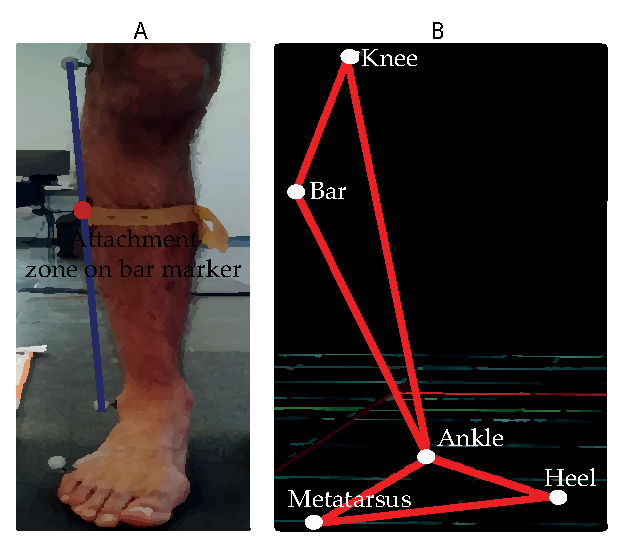
\includegraphics[width=10cm]{Markers_position.eps}
\caption{This is a figure}
\end{figure}   

\begin{figure}[H]
\centering
\includegraphics[width=10cm]{LRF_BTS_Origin.eps}
\caption{This is a figure}
\end{figure}   

\begin{figure}[H]
\centering
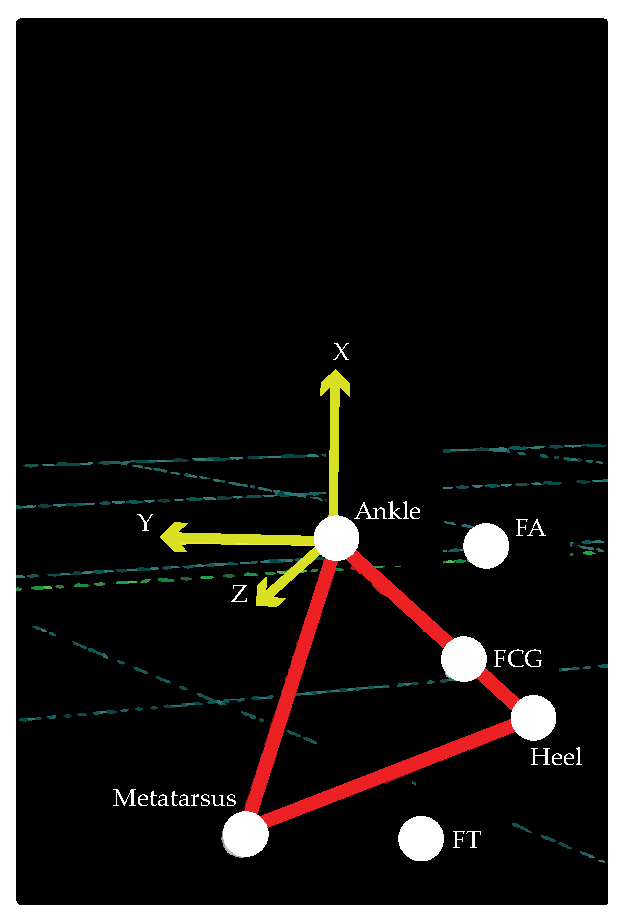
\includegraphics[width=10cm]{Foot_center_gravity.eps}
\caption{This is a figure}
\end{figure}   

\begin{figure}[H]
\centering
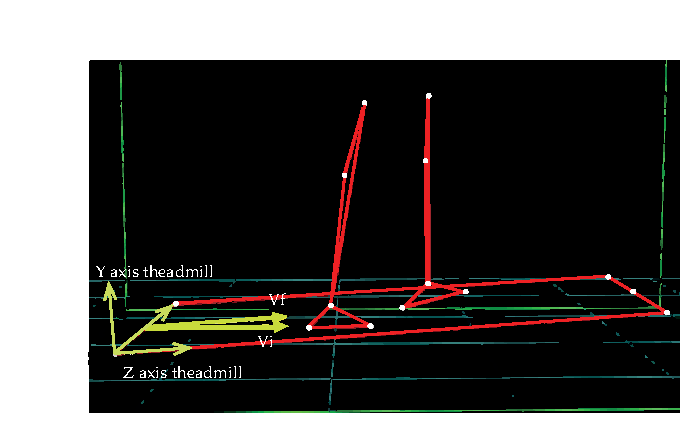
\includegraphics[width=10cm]{Inclinacion_Bandasinfin.eps}
\caption{This is a figure}
\end{figure}

\begin{figure}[H]
\centering
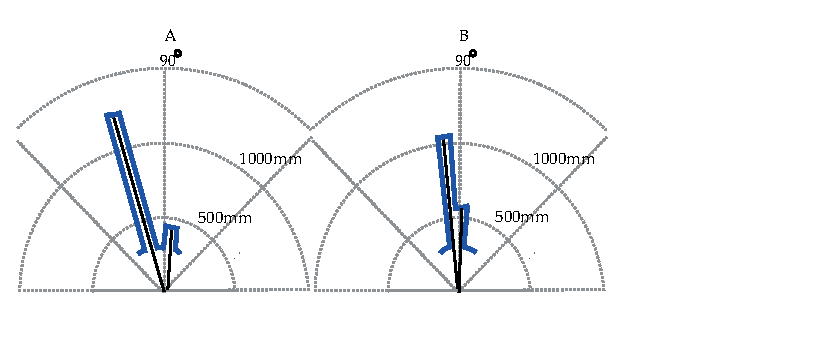
\includegraphics[width=10cm]{Legs_detection.eps}
\caption{This is a figure}
\end{figure}  

\begin{figure}[H]
\centering
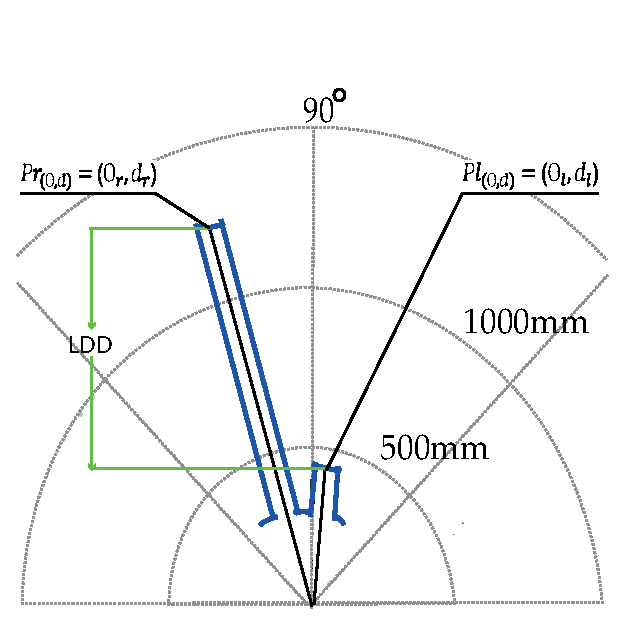
\includegraphics[width=10cm]{LDD_stimation.eps}
\caption{This is a figure}
\end{figure}   

\begin{equation}
LDD = d_{l}*sin(\theta_{l}) - d_{r}*sin(\theta_{r}) 
\end{equation}

\begin{figure}[H]
\centering
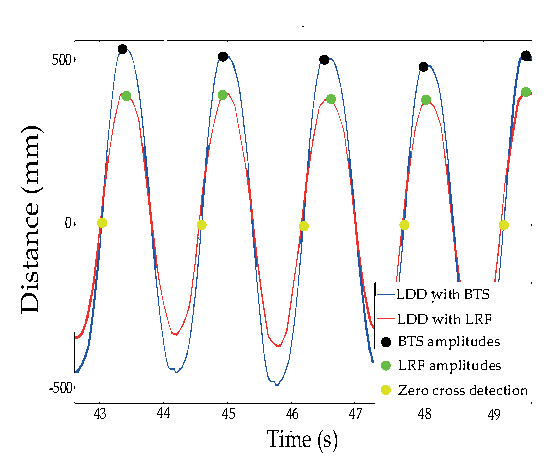
\includegraphics[width=10cm]{LDD_maxZero_detection2.eps}
\caption{This is a figure}
\end{figure} 


\subsection{Subjects}

\subsection{Materials}

\subsection{Protocol}

\subsection{data analysis}

\subsubsection{Laser range finder}

\subsubsection{Six-camera system}



%%%%%%%%%%%%%%%%%%%%%%%%%%%%%%%%%%%%%%%%%%
\section{Results}

\begin{table}[H]
\caption{Samples' Descriptive statics and results of the Wilcoxon test on the 18 initial tests without inclination (* Samples that have medians significantly different)}
\small % Font size can be changed to match table content. Recommend 10 pt.
\centering
\begin{tabular}{ccccc}
\toprule
\textbf{Treadmill speed}	& \textbf{Parameters}	& \textbf{Cameras}	& \textbf{LRF}  & \textbf{P value}\\
\midrule
1 Km/h		& Frequency	(Hz)	& $0.410 \pm 0.089$		& $0.412 \pm 0.066$		& $0.832$\\
			& Amplitude	(mm)	& $304.307 \pm 50.828$	& $264.583 \pm 40.085$	& $8.752*10^{-5*}$\\
1.8 Km/h	& Frequency	(Hz)	& $0.553 \pm 0.079$		& $0.5753 \pm 0.1487$	& $0.312$\\
			& Amplitude	(mm)	& $390.940 \pm 49.495$ 	& $322.194 \pm 41.229$	& $1.3056*10^{-7*}$\\
2.7 Km/h	& Frequency	(Hz)	& $0.646 \pm 0.080$		& $0.656 \pm 0.118$		& $0.580$\\
            & Amplitude	(mm)	& $450.696 \pm 50.616$	& $362.641 \pm 38.304$	& $3.8631*10^{-10*}$\\
3.6 Km/h	& Frequency	(Hz)	& $0.743 \pm 0.084$		& $0.735 \pm 0.099$		& $0.583$\\
            & Amplitude (mm)	& $509.400 \pm 40.887$ 	& $398.507 \pm 37.980$	& $7.3638*10^{-14*}$\\
\bottomrule
\end{tabular}
\end{table}


\begin{figure}[H]
\centering
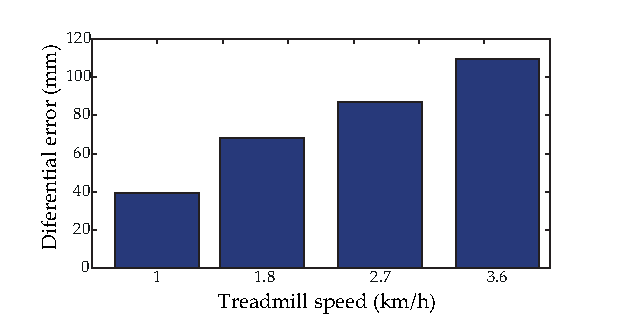
\includegraphics[width=10cm]{bar_graph_speed_vs_error.eps}
\caption{This is a figure}
\end{figure} 

\begin{equation}
K_{n} = \frac{M_{CN}}{M_{LN}}
\end{equation}


\begin{table}[H]
\caption{Frequency's mean in each speed and values of the constant K to adjust the signal's amplitude}
\small % Font size can be changed to match table content. Recommend 10 pt.
\centering
\begin{tabular}{ccc}
\toprule
\textbf{Treadmill speed (Km/h)}	& \textbf{CM (Hz)}	& \textbf{K}\\
\midrule
1 		& 0.451 	& 1.188\\
1.8		& 0.572 	& 1.225\\
2.7 	& 0.699 	& 1.245\\
3.6 	& 0.812 	& 1.2794\\

\bottomrule
\end{tabular}
\end{table}

\begin{figure}[H]
\centering
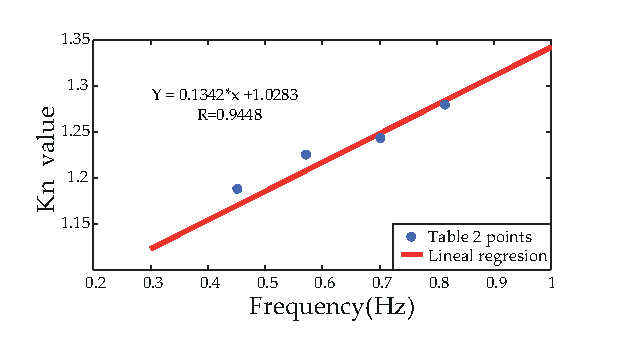
\includegraphics[width=10cm]{Kmodel.eps}
\caption{This is a figure}
\end{figure} 

\begin{equation}
K_{cadence} = 0.1343Hz^{-1}*(Cadence) + 1.0283
\end{equation}




\begin{table}[H]
\caption{Descriptive statics of the amplitudes detected (on the first group of volunteers) with the cameras' system and the LRF applying the model to adjust amplitude on LDD signals, and results of the Wilcoxon test}
\small % Font size can be changed to match table content. Recommend 10 pt.
\centering
\begin{tabular}{ccccc}
\toprule
\textbf{Treadmill speed}	& \textbf{Parameters}	& \textbf{Cameras}	& \textbf{LRF}  & \textbf{P value}\\
\midrule
1 Km/h		& Amplitude Adjusted (mm)	& $304.307 \pm 50.828$	& $310.246 \pm 44.430$	 & $0.679$\\
1.8 Km/h	& Amplitude Adjusted (mm)	& $390.940 \pm 49.495$ 	& $395.470 \pm 46.5700$	 & $0.653$\\
2.7 Km/h	& Amplitude Adjusted (mm)	& $450.696 \pm 50.616$	& $460.431 \pm 44.836$	 & $0.211$\\
3.6 Km/h	& Amplitude Adjusted (mm)	& $509.400 \pm 40.887$ 	& $512.8487 \pm 43.9151$ & $0.574$\\
\bottomrule
\end{tabular}
\end{table}

\begin{table}[H]
\caption{This is a table caption. Tables should be placed in the main text near to the first time they are cited.}
\small % Font size can be changed to match table content. Recommend 10 pt.
\centering
\begin{tabular}{ccccc}
\toprule
\textbf{Treadmill speed}	& \textbf{Parameters}	& \textbf{Cameras}	& \textbf{LRF}  & \textbf{P value}\\
\midrule
1 Km/h		& Frequency	(Hz)	& $0.5358 \pm 0.1421$	& $0.5335 \pm 0.1551$	& $0.8612$\\
			& Amplitude	(mm)	& $294.948 \pm 34.828$	& $249.659 \pm 28.249$	& $0.0020^{*}$\\
1.8 Km/h	& Frequency	(Hz)	& $0.6035 \pm 0.0933$ 	& $0.6134 \pm 0.1179$	& $0.6072$\\
			& Amplitude	(mm)	& $388.898 \pm 32.323$	& $313.322 \pm 33.836$	& $1.3257*10^{-7*}$\\
2.7 Km/h	& Frequency	(Hz)	& $0.6615 \pm 0.0851$	& $0.6661 \pm 0.0996$	& $0.7422$\\
			& Amplitude	(mm)	& $472.610 \pm 38.573$	& $365.942 \pm 41.832$	& $1.2226*10^{-9*}$\\
3.6 Km/h	& Frequency	(Hz)	& $0.7600 \pm 0.0756$ 	& $0.7572 \pm 0.0967$ 	& $0.7439$\\
			& Amplitude	(mm)	& $542.592 \pm 36.286$	& $416.863 \pm 39.197$	& $1.5641*10^{-10*}$\\
\bottomrule
\end{tabular}
\end{table}

\begin{table}[H]
\caption{This is a table caption. Tables should be placed in the main text near to the first time they are cited.}
\small % Font size can be changed to match table content. Recommend 10 pt.
\centering
\begin{tabular}{cccc}
\toprule
\textbf{Treadmill speed (Km/h)}	& \textbf{Amplitude using cameras  (mm)}	& \textbf{Amplitude adjusted using LRF (mm)} & \textbf{P value}\\
\midrule
1 		& $294.948 \pm 34.828$		& $293.597 \pm 29.428$ 	& $0.9218$\\
1.8		& $388.898 \pm 32.323$		& $383.189 \pm 39.339$ 	& $0.8457$\\
2.7 	& $472.609 \pm 38.573$		& $461.509 \pm 47.787$ 	& $0.5703$\\
3.6 	& $542.592 \pm 36.286$		& $539.664 \pm 46.208$ 	& $0.7960$\\

\bottomrule
\end{tabular}
\end{table}


\begin{figure}[H]
\centering
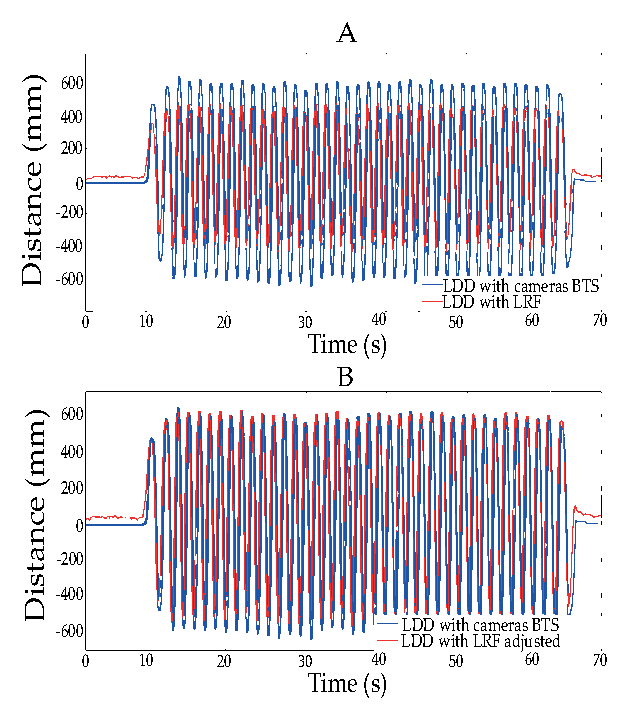
\includegraphics[width=10cm]{LDD_coparation.eps}
\caption{This is a figure}
\end{figure} 



\begin{table}[H]
\caption{This is a table caption. Tables should be placed in the main text near to the first time they are cited.}
\small % Font size can be changed to match table content. Recommend 10 pt.
\centering
\begin{tabular}{ccccc}
\toprule
\textbf{Treadmill speed}	& \textbf{Parameters}	& \textbf{Cameras}	& \textbf{LRF}  & \textbf{P value}\\
\midrule
1 Km/h		& Frequency	(Hz)	& $0.4479 \pm 0.0704$	& $0.4509 \pm 0.0695$	& $0.3036$\\
			& Amplitude	(mm)	& $365.429 \pm 55.134$	& $307.596 \pm 37.492$	& $1.82*10^{-5*}$\\
1.8 Km/h	& Frequency	(Hz)	& $0.5698 \pm 0.0569$ 	& $0.5716 \pm 0.0595$	& $0.3532$\\
			& Amplitude	(mm)	& $454.578 \pm 48.606$	& $358.824 \pm 41.692$	& $1.22*10^{-5*}$\\
2.7 Km/h	& Frequency	(Hz)	& $0.6911 \pm 0.0620$	& $0.6985 \pm 0.0594$	& $0.6553$\\
			& Amplitude	(mm)	& $534.603 \pm 42.882$	& $416.796 \pm 39.615$	& $5.95*10^{-5*}*$\\
3.6 Km/h	& Frequency	(Hz)	& $0.7960 \pm 0.0655$ 	& $0.8007 \pm 0.0539$ 	& $0.0945$\\
			& Amplitude	(mm)	& $597.837 \pm 40.449$	& $ 460.653 \pm 43.004$	& $4.01*10^{-5*}*$\\
\bottomrule
\end{tabular}
\end{table}

\begin{table}[H]
\caption{This is a table caption. Tables should be placed in the main text near to the first time they are cited.}
\small % Font size can be changed to match table content. Recommend 10 pt.
\centering
\begin{tabular}{cccc}
\toprule
\textbf{Treadmill speed (Km/h)}	& \textbf{Amplitude using cameras  (mm)}	& \textbf{Amplitude adjusted using LRF (mm)} & \textbf{P value}\\
\midrule
1 		& $365.429 \pm 55.134$	& $359.824 \pm 47.274$ & $0.8864$\\
1.8		& $454.578 \pm 48.606$	& $446.002 \pm 42.181$ & $0.1742$\\
2.7 	& $534.603 \pm 42.882$	& $522.621 \pm 43.694$ & $0.1084$\\
3.6 	& $597.837 \pm 40.449$	& $593.009 \pm 46.450$ & $0.8328$\\

\bottomrule
\end{tabular}
\end{table}


\begin{figure}[H]
\centering
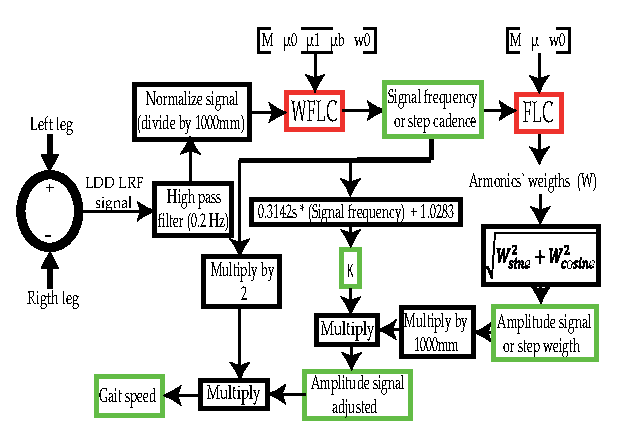
\includegraphics[width=10cm]{Diagram_Model.eps}
\caption{This is a figure}
\end{figure} 

\begin{figure}[H]
\centering
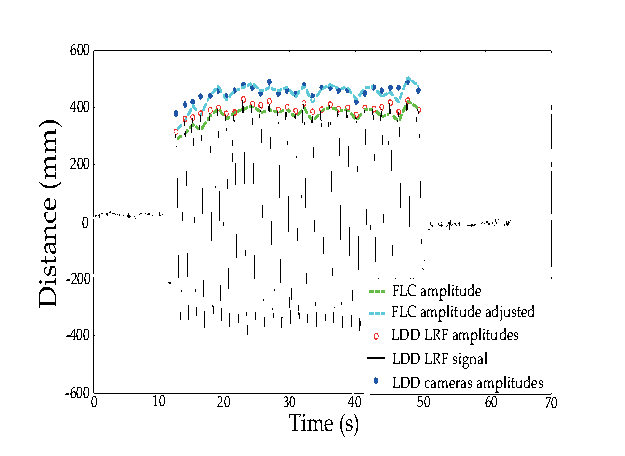
\includegraphics[width=10cm]{AmplitudeFLC_Adjusted.eps}
\caption{This is a figure}
\end{figure} 

\begin{figure}[H]
\centering
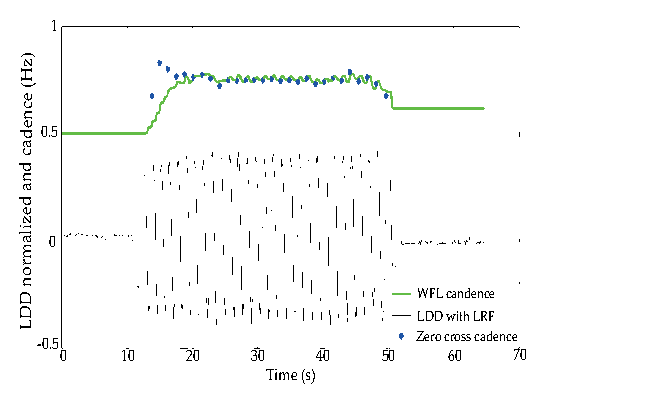
\includegraphics[width=10cm]{CadenceWFLC.eps}
\caption{This is a figure}
\end{figure} 

\begin{table}[H]
\caption{This is a table caption. Tables should be placed in the main text near to the first time they are cited.}
\small % Font size can be changed to match table content. Recommend 10 pt.
\centering
\begin{tabular}{ccccc}
\toprule
\textbf{Treadmill speed}	& \textbf{Parameters}	& \textbf{Cameras}	& \textbf{LRF applying WFLC and  FLC with the adjustment}  & \textbf{P value}\\
\midrule
1 Km/h		& Frequency	(Hz)	& $0.4110 \pm 0.0594$	& $0.4051 \pm 0.060$	& $0.8927$\\
			& Amplitude	(mm)	& $300.019 \pm 45.885$	& $311.897 \pm 67.435$	& $0.5878$\\
1.8 Km/h	& Frequency	(Hz)	& $0.5673 \pm 0.0442$ 	& $0.5823 \pm 0.0289$	& $0.1858$\\
			& Amplitude	(mm)	& $384.577 \pm 43.523$	& $385.907 \pm 52.523$	& $0.4565$\\
2.7 Km/h	& Frequency	(Hz)	& $0.6910 \pm 0.0535$	& $0.6908 \pm 0.0458$	& $0.8039$\\
			& Amplitude	(mm)	& $453.444 \pm 48.858$	& $443.678 \pm 70.215$	& $0.3302$\\
3.6 Km/h	& Frequency	(Hz)	& $0.7947 \pm 0.0460$ 	& $0.7844 \pm 0.0295$ 	& $0.6848$\\
			& Amplitude	(mm)	& $513.233 \pm 43.193$	& $514.158 \pm 76.164$	& $0.9460$\\
\bottomrule
\end{tabular}
\end{table}



%% If the documentclass option "submit" is chosen, please insert a blank line before and after any math environment (equation and eqnarray environments). This ensures correct linenumbering. The blank line should be removed when the documentclass option is changed to "accept" because the text following an equation should not be a new paragraph. 
Please punctuate equations as regular text. Theorem-type environments (including propositions, lemmas, corollaries etc.) can be formatted as follows:
%% Example of a theorem:
\begin{Theorem}
Example text of a theorem.
\end{Theorem}
The text continues here. Proofs must be formatted as follows:

%% Example of a proof:
\begin{proof}[Proof of Theorem 1]
Text of the proof. Note that the phrase `of Theorem 1' is optional if it is clear which theorem is being referred to.
\end{proof}
The text continues here.

%%%%%%%%%%%%%%%%%%%%%%%%%%%%%%%%%%%%%%%%%%
\section{Discussion}

This section may be divided by subheadings. Authors should discuss the results and how they can be interpreted in perspective of previous studies and of the working hypotheses. The findings and their implications should be discussed in the broadest context possible. Future research directions may also be highlighted.


%%%%%%%%%%%%%%%%%%%%%%%%%%%%%%%%%%%%%%%%%%
\section{Conclusions}

This section is not mandatory, but can be added to the manuscript if the discussion is unusually long or complex.

%%%%%%%%%%%%%%%%%%%%%%%%%%%%%%%%%%%%%%%%%%
\vspace{6pt} 

%%%%%%%%%%%%%%%%%%%%%%%%%%%%%%%%%%%%%%%%%%
%% optional
\supplementary{The following are available online at www.mdpi.com/link, Figure S1: title, Table S1: title, Video S1: title.}

%%%%%%%%%%%%%%%%%%%%%%%%%%%%%%%%%%%%%%%%%%
\acknowledgments{All sources of funding of the study should be disclosed. Please clearly indicate grants that you have received in support of your research work. Clearly state if you received funds for covering the costs to publish in open access.}

%%%%%%%%%%%%%%%%%%%%%%%%%%%%%%%%%%%%%%%%%%
\authorcontributions{For research articles with several authors, a short paragraph specifying their individual contributions must be provided. The following statements should be used ``X.X. and Y.Y. conceived and designed the experiments; X.X. performed the experiments; X.X. and Y.Y. analyzed the data; W.W. contributed reagents/materials/analysis tools; Y.Y. wrote the paper.'' Authorship must be limited to those who have contributed substantially to the work reported.}

%%%%%%%%%%%%%%%%%%%%%%%%%%%%%%%%%%%%%%%%%%
\conflictofinterests{Declare conflicts of interest or state ``The authors declare no conflict of interest.'' Authors must identify and declare any personal circumstances or interest that may be perceived as inappropriately influencing the representation or interpretation of reported research results. Any role of the funding sponsors in the design of the study; in the collection, analyses or interpretation of data; in the writing of the manuscript, or in the decision to publish the results must be declared in this section. If there is no role, please state ``The founding sponsors had no role in the design of the study; in the collection, analyses, or interpretation of data; in the writing of the manuscript, and in the decision to publish the results''.} 

%%%%%%%%%%%%%%%%%%%%%%%%%%%%%%%%%%%%%%%%%%
%% optional
\abbreviations{The following abbreviations are used in this manuscript:\\

\noindent MDPI: Multidisciplinary Digital Publishing Institute\\
DOAJ: Directory of open access journals\\
TLA: Three letter acronym\\
LD: linear dichroism}

%%%%%%%%%%%%%%%%%%%%%%%%%%%%%%%%%%%%%%%%%%
%% optional
\appendix
\section{}
The appendix is an optional section that can contain details and data supplemental to the main text. For example, explanations of experimental details that would disrupt the flow of the main text, but nonetheless remain crucial to understanding and reproducing the research shown; figures of replicates for experiments of which representative data is shown in the main text can be added here if brief, or as Supplementary data. Mathemtaical proofs of results not central to the paper can be added as an appendix.

\section{}
All appendix sections must be cited in the main text. In the appendixes, Figures, Tables, etc. should be labeled starting with `A', e.g., Figure A1, Figure A2, etc. 

%%%%%%%%%%%%%%%%%%%%%%%%%%%%%%%%%%%%%%%%%%
\bibliographystyle{mdpi}

%=====================================
% References, variant A: internal bibliography
%=====================================
\renewcommand\bibname{References}
\begin{thebibliography}{999}
% Reference 1
\bibitem{ref-journal}
Lastname, F.; Author, T. The title of the cited article. {\em Journal Abbreviation} {\bf 2008}, {\em 10}, 142-149.
% Reference 2
\bibitem{ref-book}
Lastname, F.F.; Author, T. The title of the cited contribution. In {\em The Book Title}; Editor, F., Meditor, A., Eds.; Publishing House: City, Country, 2007; pp. 32-58.
\end{thebibliography}

%=====================================
% References, variant B: external bibliography
%=====================================
%\bibliography{your_external_BibTeX_file}

%%%%%%%%%%%%%%%%%%%%%%%%%%%%%%%%%%%%%%%%%%
%% optional
\sampleavailability{Samples of the compounds ...... are available from the authors.}

%%%%%%%%%%%%%%%%%%%%%%%%%%%%%%%%%%%%%%%%%%
\end{document}

